\section{Discussion}

Systems like Google and StackOverflow already satisfy users' queries.
However, learning a new workflow or procedure with new libraries is still challenging for programmers.
One cause of this is the new vocabulary required.
The other is the short time frame and high expectations programmers have of training material.
\Glspl{name} does not seek to replace existing search solutions that provide great answers in a short amount of time.
They aim to make online tutorials for acquiring more skills more relevant when correcting errors and adapting tutorial code to personal tasks.

In the future, we plan to explore the \Glspl{name} ecosystem in more depth.
We can investigate alternate techniques for detecting \emph{skills assumed} in tutorials.
This can be extended beyond programming-based skills to other concepts, leveraging document-linking strategies like that described by Milne \& Witten for linking Wikipedia resources~\cite{milne_learning_2008}.
In line with detecting non-programming content types, we would also want to explore ways of automatically describing these content types.

A system like \Glspl{name} can be implemented as a browser extension.
Such an extension can maintain a memory of everywhere a user has been, online coding activites they have performed, and past \glspl{name} that they have accessed.
We see this as a rich space for developing approximations of online learners' knowledge models.
After developing such models, we would like to explore how to better automatically adapt existing in-the-wild web resources to programming learners' current capabilities and information seeking habits.

There are some caveats from our user studies.
For the preliminary investigation, this includes A.
For the informal usability study, this includes B.
For the formal in-lab study, this includes C.

Ultimately, we see a future where documents and community-sourced feedback can be quickly and, in some cases, automatically connected to make more usable documentation for users that need to rapidly acquire new skills.
While Wikipedia has started this vision with densely hyperlinked pages, we believe this is only one way to connect resources, and is currently applied only to a closed set of documents.
\Glspl{name} represent and exploratory step towards more seamless integration of disparate documentation and application of community-sourced knowledge across the wild web of learning resources.

\section{Design Space}

In its current form, \glspl{name} can support simple grammars.
It supports authoring and well as comprehension tasks (Figure~\ref{fig:design_space}).
The users in the \glspl{name} ecosystem are developers writing adaptive documentation, authors of tutorial content, or readers of tutorials.

\begin{figure}
\centering{
    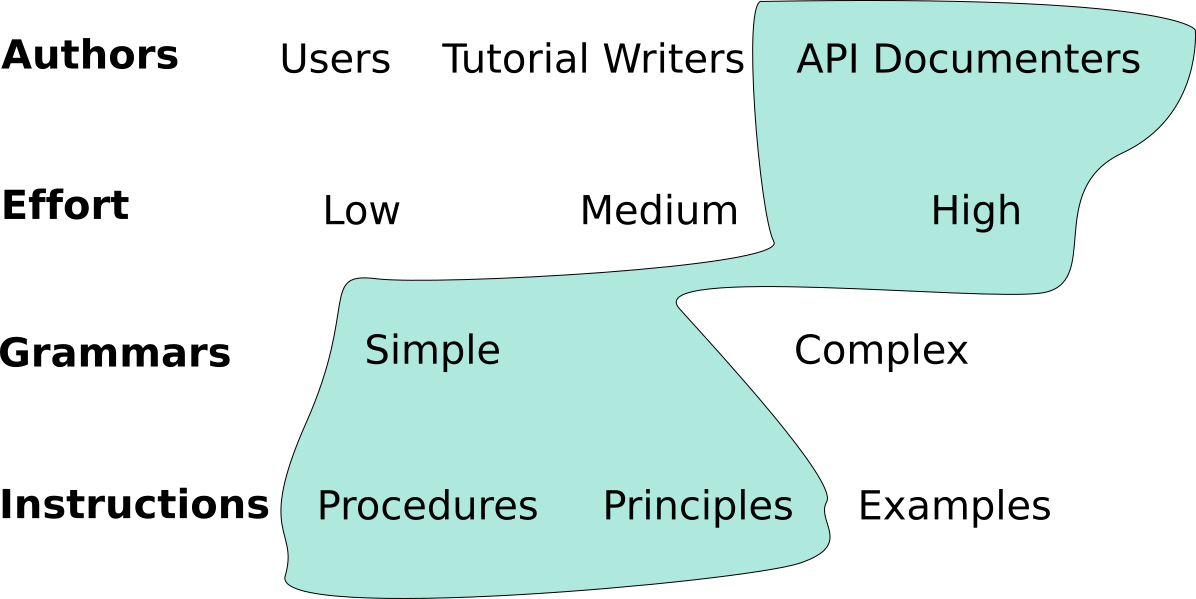
\includegraphics[width=.4\textwidth]{figures/design_space}
}
\caption{
The design space of \glspl{name}.  We highlight in color the portion of the design space that we consider in this paper.
\andrew{This design space is supposed to highlight principles and examples, but not procedures in the instructions row.}
}
\label{fig:design_space}
\end{figure}

\section{Implementation}

Custom were written in ANTLR\footnote{\url{http://www.antlr.org/}} (wget, CSS).
External libraries generate descriptions\footnote{\url{http://rick.measham.id.au/paste/explain.pl}} and visualizations\footnote{\url{http://regexper.com/}} of regular expressions.
We use the SimpleNLG\footnote{\url{https://code.google.com/p/simplenlg/}} Java library to generate natural language descriptions.
Descriptions are served up via servers written in Django\footnote{\url{https://www.djangoproject.com/}}.
We develop the Firefox addon with the Firefox Add-Ons API\footnote{\url{https://developer.mozilla.org/en-US/Add-ons/SDK}}.
